\section{Solarzelle}

\subsection*{Funktionsprinzip einer Solarzelle}
Durch Einstrahlung von Photonen werden freie Ladungsträger in der Zelle erzeugt. Der p-n-Übergang erzeugt ein inneres elektrisches Feld. Das herausgelöste Elektron und das entstandene Loch werden dadurch in unterschiedliche Richtungen transportiert. Hieraus entsteht ein Strom.\\
Das herauslösen eines Elektrons ist nur möglich, wenn die Energie $E=hv$ größer der Gap-Energie des Halbleitermaterials ist.

\subsection*{Füllfaktor}
Das Verhältnis zwischen theoretisch erzielbarer Leistung und der am Maximum Power Point (MPP) erzielten Leistung, wird Füllfaktor genannt. 
Abb. \ref{fuell} zeigt den Füllfaktor grafisch.
\begin{figure}[htb]
	\centering
	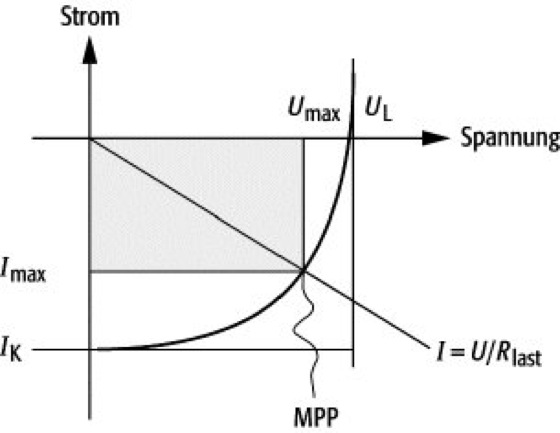
\includegraphics[width=0.7\textwidth]{Abb/fuellfaktor.jpg}
	\caption{Der Füllfaktor grafisch}
	\label{fuell}
\end{figure}

\subsection*{Wärmeeinwirkung auf Solarzelle}
Die Anzahl der freien Ladungsträger nimmt im Halbleiter mit der Temperatur zu. Diese Ladungsträger bewirken in der Sperrschicht der Solarzelle einen Diffusionsstrom, der die Leistung der Solarzelle reduziert.

\subsection*{Effizienz der Solarzelle}
Die Effizienz hängt neben den offensichtlichen Faktoren, wie Wellenlänge/Spektrum des eingestrahlten Lichts, und der oben genannten Wärmeabhängigkeit, noch von Bauart bedingten Einschränkungen ab. Hier seien die Dicke der Schichten der Photozelle und dem Material gennant. 
Von den in \ref{halbmatt} genannten Materialien, weißt zum Beispiel kristallines Silizium eine höhere Effizienz auf, als amorphes. Weiter werden in Raumfahrtanwendungen sehr teure Materialien wie GaAs, oder GaAlAs und GaInAsP, verwendet, die Effizienzen bist 40\% erreichen.

\begin{figure}[htb]
	\centering
	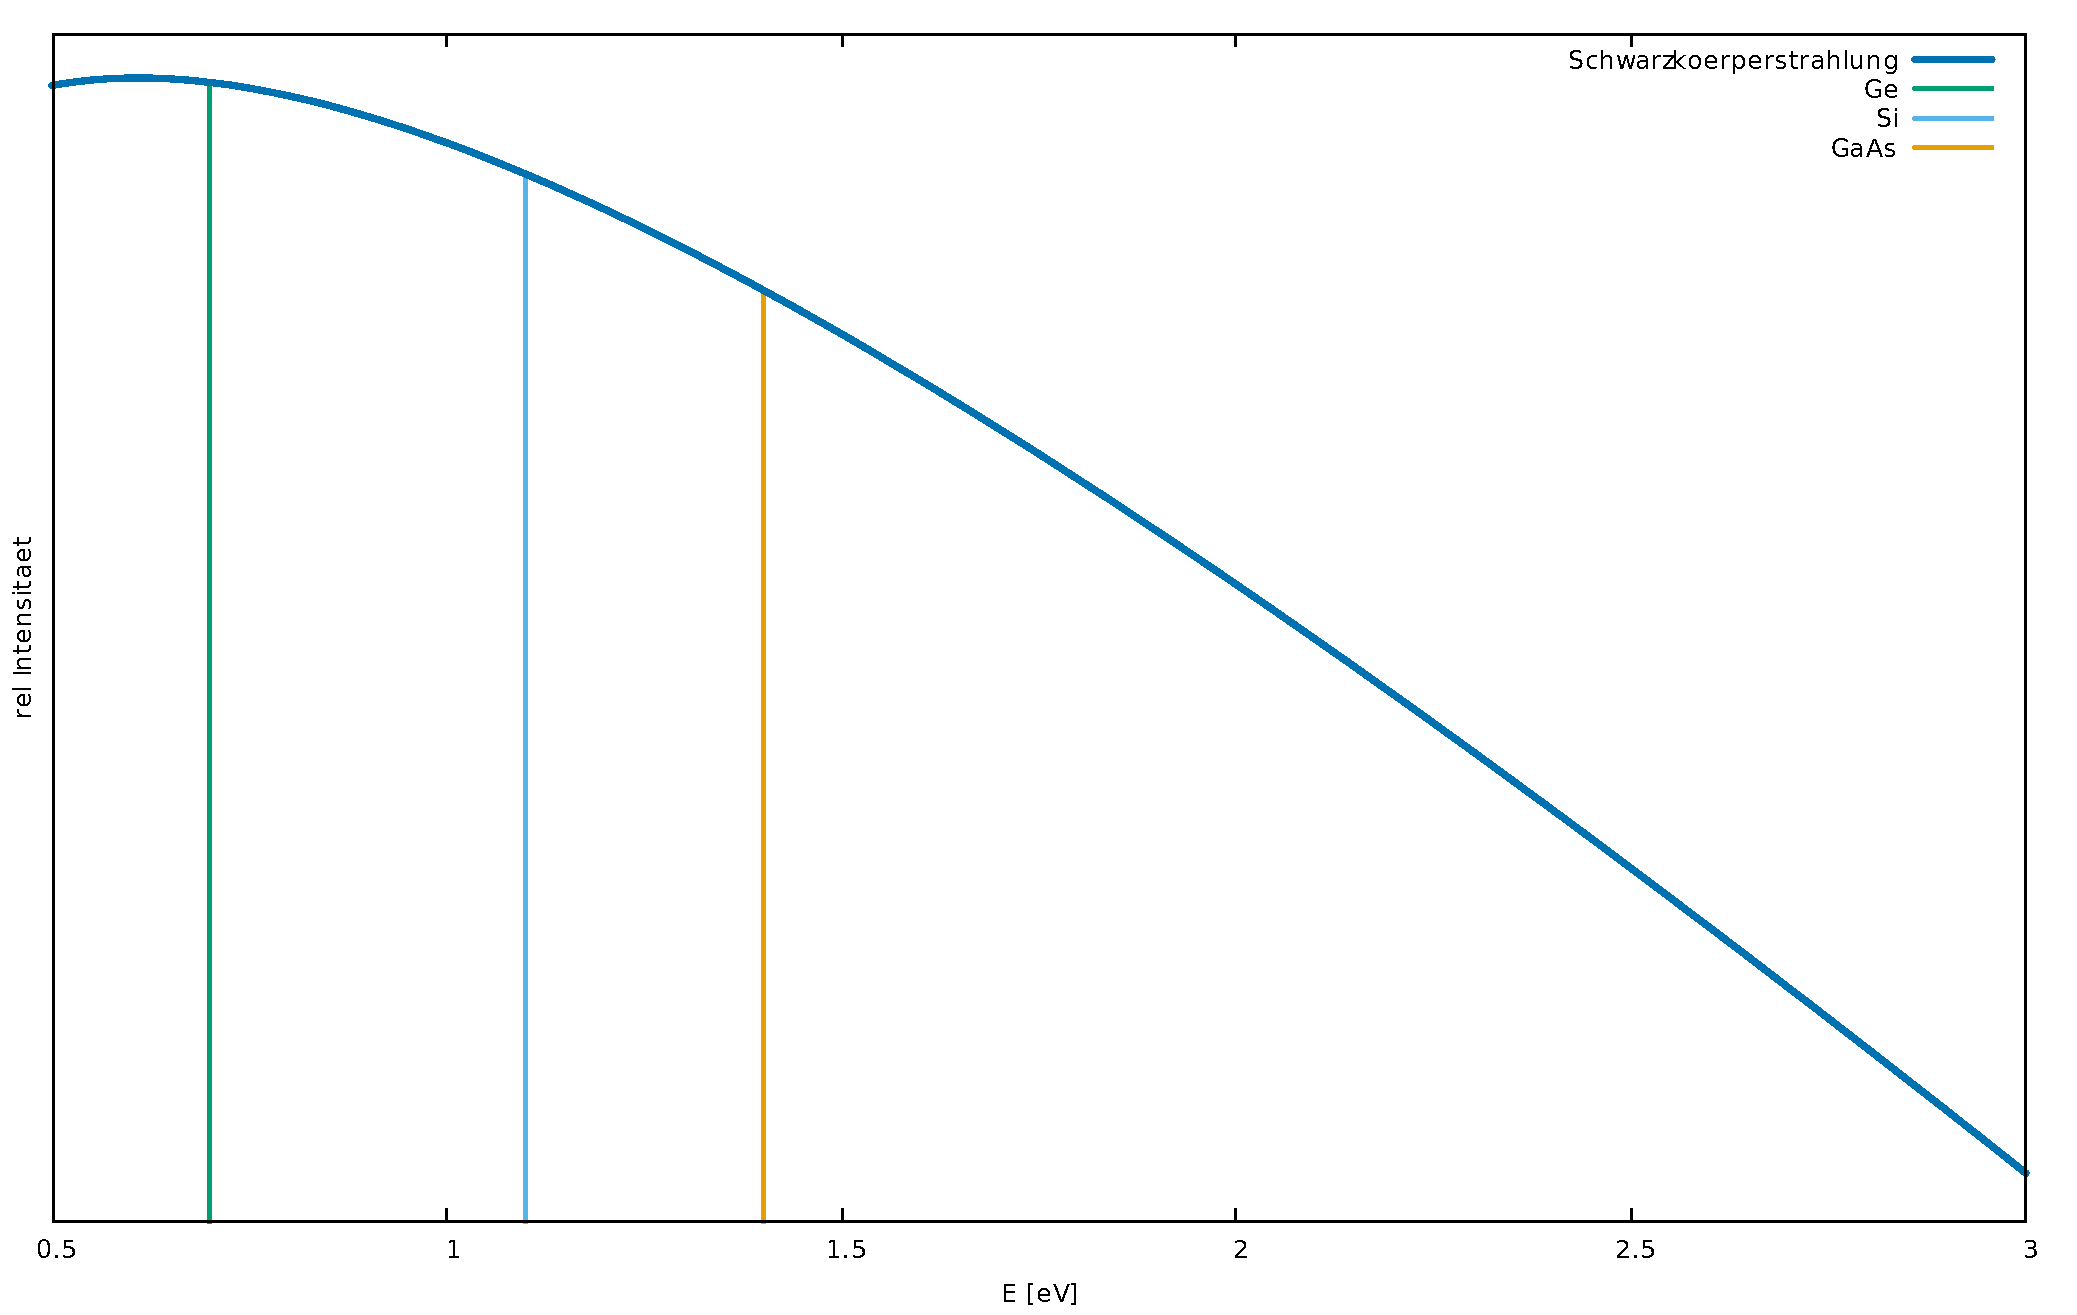
\includegraphics[width=0.8\textwidth]{Abb/aufg18.pdf}
	\caption{Intensität eines schwarzen Strahlers mit 2500K, Gapenergien einiger typischer Halbleiterverbindungen}
	\label{aufg18}
\end{figure}
\subsection*{Spektrum des schwarzen Strahlers}
Abb. \ref{aufg18} zeigt die Strahlung eines schwarzen Strahlers bei 2500K in Abhängigkeit der Energie der emittierten Photonen, sowie die Gapenergie verschiedener Halbleiter. Der Anteil der Strahlung rechts von den Strichen trägt zur Leistung der Solarzelle bei.

\subsection*{Abhängigkeit des Fotostroms von der Temperatur des schwarzen Strahlers}
Die Anzahl der erzeugten Elektron-Loch-Paare ist proptoortional zur Anzahl der Photonen, die eine Energie größer der Gap-Energie besitzen. Der Anteil dieser Photonen lässt sich mit dem Wien'schen Verschiebungsgesetz bestimmen. 
\[
M( \lambda ) = \frac{2 \pi c^2}{ \lambda^5 } \frac{ 1 }{ \exp \left( \frac{hc}{k_B T} \right) }
\]
mit $\lambda = c/v$ und $E_{Gap} = hv$ folgt:
\[
M(v) = \frac{2 \pi v^5}{c^3} \frac{1}{ \exp \left( \frac{E_{Gap}}{k_B T} \right)}
\]
Für die Intensität gilt
\[
I \propto \frac{2 \pi v^5}{c^3} \frac{1}{ \exp \left( \frac{E_{Gap}}{k_B T} \right)} \propto \exp \left( - \frac{E_{Gap}}{k_B T} \right)
\]
